\section{Software}
Die Software bildet den wichtigsten Teil des Bindeglieds zwischen Benutzer und Hardware. Als erstes muss den Sensorplatinen eine Indentifikationsnummer zugeteilt und in der Zentrale die Anzahl Module angegeben werden. Die Gemessenen Spannungswerte der Solarmodule werden via Powerline an die Meldeplatine gesendet. Es sollen keine extra Datenkabel verwendet werden. Diese Daten müssen in der Meldezentrale verarbeitet werden. Eine allfällige Abweichung des Spannungswertes bei einem oder mehreren Modulen sollen erkannt und identifiziert werden. Worin genau diese Abweichung besteht, wird später erläutert. Nach der Identifikation muss ein solcher Fehler gemeldet werden. Die Kommunikation zwischen Hardware und Software basiert auf SPI. Das Endprodukt setzt aus dem Melde- und Sensor-Print zusammen. In dieser Unterteilung werden in den nächsten Kapiteln alle Softwarekomponenten beschrieben.
\subsection{Sensorprint}
Der Sensorprint übernimmt die Spannungsmessung und sendet diese mit der Identifikationsnummer via Powerline an den Meldeprint. Die Kopplung in die Powerline gelingt mit einem Ferritkern. In den folgenden Kapiteln wird die Software weiter unterteilt und jeder Bereich einzeln erläutert.
\subsubsection{Aufbau und Abläufe}
Der Aufbau der Software auf der Sensorplatine basiert auf zwei verschiedenen Kommunikationsprotokollen. Zwischen dem ADC und dem Mikrocontroller via SPI und dem Mikrocontroller und dem Tranceiver via UART. In der Abbildung \ref{DiagrammSP} ist der Ablauf der Software dargestellt.
\begin{figure}
\centering
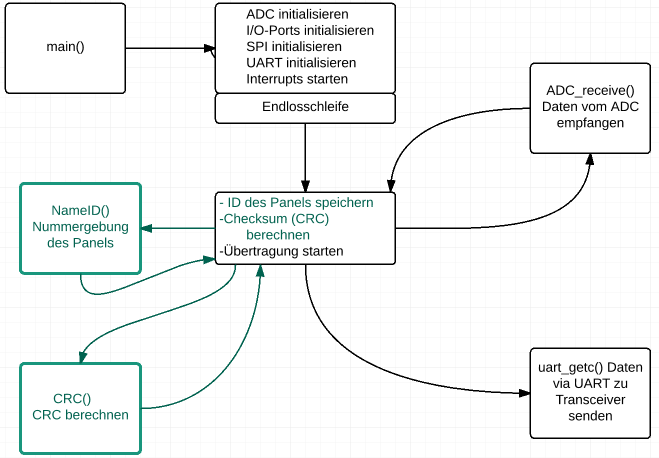
\includegraphics[width=0.6\textwidth]{data/Sensorplatine}
\label{DiagrammSP}
\end{figure}
In der vorhergehenden Abbildung ist der Zusammenhang der einzelnen Teilprogramme ersichtlich. Wird das main() aufgerufen werden die Teilprogramme in der Endlosschlaufe aufgerufen.
\subsubsection{Inbetriebnahme}
Die Identifikationsnummer kann über das Einlesen der Schalter gespeichert bzw. definiert werden. Dies muss vom Benutzer eindeutig und selbständig eingestellt werden. Der Plan ist, dass man via USB dem Panel zusätzlich ein Name gegeben werden kann.
\subsubsection{Spannungsmessung}
%wieso-was-wie-unter welchen Bedingungen
Die Kommunikation zwischen ADC und Mikrocontroller basiert auf dem Master-Salve-Prinzip. Der Plan ist, dass die empfangenen Werte vom ADC vom Mikrocontroller in einem bestimmten Zeitraum gespeichert gespeichert werden und der Mittelwert weiter an den Transceiver geleitet wird.\\
Als Basis für die Spannungsmessung soll zukünftig ein Referenzwert dienen. Der empfangene Wert soll durch Berechnung der Abweichung zu diesem Referenzwert dem Spannnungswert zugeteilt werden. Schlussendlich soll der durchschnittliche Spannungswert weiter an den Transceiver geleitet werden.
\subsubsection{Transceiveransteuerung}
%wieso-was-wie-unter welchen Bedingungen
















\newpage
\subsection{Meldeprint}
Der Meldeprint empfängt die Daten des Sensorprints mit Hilfe eines Receivers. Die Spannungswerte werden in Verbindung mit der Identifikationsnummer gespeichert und mit dem Sollwert vergleicht. Der Sollwert entspricht dem arithmetischen Mittelwert der Spannungen dieses einen Strings von Modulen. Bei einer Abweichung von mehr als 20 Prozent von der Standardabweichung, wird dasjenige Modul vorgemerkt. Falls nach einer weiteren Messung die Spannung des selben Moduls gleich vom Mittelwert abweicht, muss ein Fehler gemeldet werden. Die Identifikationsnummer wird auf dem Display angezeigt. Die in Standard C geschriebene Software bezieht sich auf den ATMEGA328P von Atmel. Das Hauptprogramm beinhaltet die Initialisierungen der Pins, des LCD Display, des Transceivers und des Drehgebers.Die einzelnen Bereiche werden unten genauer erläutert.
\subsubsection{Aufbau und Abläufe (Flussdiagramm)}
\subsubsection{Inbetriebnahme}

Der Meldeprint

Bei der Inbetriebnahme werden als erstes die Peripheriegeräte initialisiert. Darunter befinden sich der LC Display und der Receiver \todo{ist die uart kommunikation der receiver?}. Weiter muss die UART Kommunikation und der Timer Interrupt initialisiert werden. In der Endlosschlaufe des Hauptprogramms werden dann die Daten der Sensorplatine in einem Array Register gespeichert und weiterverarbeitet.

\subsubsection{Receiver}
Der Receiver detektiert über einen Ferrit-Kern über der DC-Leitung des Strings die Signale der Sensorplatine. Die Datenpakete werden mit der Identifikationsnummer an den Arduino weitergeleitet über die UART Kommunikation.
\subsubsection{Fehlererkennung}
Aus Zeitgründen konnte die Datenverarbeitung noch nicht programmiert werden. Der Plan ist aber die gemittelten Spannungswerte, die jede Sensorplatine liefert, nochmals über alle Module des Strings zu mitteln. Damit kann dann die Standardabweichung berechnet werden. Ist die Abweichung eines Wertes mehr als 20 Prozent über der Standardabweichung, wird diese Solarmodul vorgemerkt. Diese Prozedere wiederholt sich stündlich. Weicht der Spannungswert des vorgemerkten Moduls nach der nächsten Stunde noch immer so stark vom Mittelwert ab, wird eine Fehlermeldung losgeschickt.

wieso-was-wie-unter welchen Bedingungen
\subsubsection{Fehlermeldung (Display und Relais)}
Die Fehlermeldung besteht aus der Fehlerankündigung selbst und der Identifikationsnummer der Sensorplatine, welche am defekten oder verschmutzten Modul befestigt ist. Die Fehlerankündigung ist als Text wie beispielsweise "Problem beim Modul..." auf dem Display zu sehen. Die Identifikationsnummer des Moduls wird von einer 8bit Binärzahl in eine Dezimalzahl umgewandelt und so angezeigt.

wieso-was-wie-unter welchen Bedingungen
\subsubsection{Benutzerinterface (Display und Drehgeber)}

Das Menü und der Drehgeber bilden zusammen eine einfache Schnittstelle zwischen Mensch und Maschine. Das Menü ist in drei Ebenen unterteilt welche in Abbildung \todo{Abbildung Menü} dargestellt ist.


